\providecommand{\rupee}{Rs.}
\emergencystretch=3em
\renewcommand{\vec}[1]{#1}
\renewcommand{\solution}{\noindent Solution: }
\begin{enumerate}[label=\thesubsection.\arabic*, ref=\thesubsection.\theenumi, itemsep=3ex]
%--------------------------------------------------------------------- Section A

\item
Write the value of $\cot\brak{\tan^{-1}a + \cot^{-1}a}$.

\smallskip
\solution From \eqref{eq:EE26BTECH11205-tan-cot},
\begin{align}
	\cot\brak{\tan^{-1}a + \cot^{-1}a} = \cot\frac{\pi}{2} = 0
\end{align}

\item
If $\vec{A}$ is a square matrix such that $\vec{A}^2 = \vec{A}$, then write the value of $\brak{\vec{I}+\vec{A}}^2 - 3\vec{A}$.

\smallskip
\solution From \eqref{eq:EE26BTECH11205-idem-binom} and $\vec{A}^2 = \vec{A}$,
\begin{align}
	\brak{\vec{I}+\vec{A}}^2 - 3\vec{A} = \vec{I} + 2\vec{A} + \vec{A} - 3\vec{A} = \vec{I}
\end{align}
The following code verifies the solution using a random idempotent matrix
\begin{lstlisting}[frame=single, basicstyle=\rmfamily, escapeinside={(*@}{@*)}]
(*@\makebox[\dimexpr\linewidth-2\fboxsep-2\fboxrule\relax][c]{codes/Q02.py}@*)
\end{lstlisting}

\item
If $x\myvec{2 \\ 3} + y\myvec{-1 \\ 1} = \myvec{10 \\ 5}$, write the value of $x$.

\smallskip
\solution The equation can be expressed as
\begin{align}
	\myvec{2 & -1 \\ 3 & 1}\myvec{x \\ y} = \myvec{10 \\ 5}
\end{align}
The determinant of the coefficient matrix is $2\brak{1} - \brak{-1}\brak{3} = 5 \neq 0$. From \eqref{eq:EE26BTECH11205-linsys},
\begin{align}
	\myvec{x \\ y} = \frac{1}{5}\myvec{1 & 1 \\ -3 & 2}\myvec{10 \\ 5} = \frac{1}{5}\myvec{15 \\ -20} = \myvec{3 \\ -4}
\end{align}
Hence $x = 3$ (and $y = -4$).

\smallskip
The following code verifies the solution
\begin{lstlisting}[frame=single, basicstyle=\rmfamily, escapeinside={(*@}{@*)}]
(*@\makebox[\dimexpr\linewidth-2\fboxsep-2\fboxrule\relax][c]{codes/Q03.py}@*)
\end{lstlisting}

\item
Write the value of the following determinant:
\begin{align}
	\mydet{102 & 18 & 36 \\ 1 & 3 & 4 \\ 17 & 3 & 6}
\end{align}

\smallskip
\solution
Let $\vec{R}_i$ denote the $i^{\text{th}}$ row. Then
\begin{align}
	\vec{R}_1 = \myvec{102 & 18 & 36} = 6\myvec{17 & 3 & 6} = 6\vec{R}_3
\end{align}
The row operation $\vec{R}_1 \to \vec{R}_1 - 6\vec{R}_3$ gives a zero row. From \eqref{eq:EE26BTECH11205-det-prop}, the determinant is $0$.

\item
If $\int\brak{\frac{x-1}{x^2}}e^x\,dx = f(x)e^x + c$, then write the value of $f(x)$.

\smallskip
\solution Write
\begin{align}
	\frac{x-1}{x^2} = \frac{1}{x} - \frac{1}{x^2} = g(x) + g^{\prime}(x),\quad g(x) = \frac{1}{x}
\end{align}
From \eqref{eq:EE26BTECH11205-exp-int},
\begin{align}
	\int\brak{\frac{x-1}{x^2}}e^x\,dx = \frac{e^x}{x} + c
\end{align}
Hence $f(x) = \frac{1}{x}$.

\item
Write the value of the area of the parallelogram determined by the vectors $2\hat{\imath}$ and $3\hat{\jmath}$.

\smallskip
\solution From \eqref{eq:EE26BTECH11205-area-gram}, with the vectors taken in the $xy$-plane,
\begin{align}
	\vec{a} = \myvec{2 \\ 0}, \quad \vec{b} = \myvec{0 \\ 3}
	\\
	\vec{M} = \myvec{\vec{a} & \vec{b}} = \myvec{2 & 0 \\ 0 & 3}
	\\
	\text{Area} &= \sqrt{\det\brak{\vec{M}^{\top}\vec{M}}} = \sqrt{\mydet{\vec{a}^{\top}\vec{a} & \vec{a}^{\top}\vec{b} \\ \vec{b}^{\top}\vec{a} & \vec{b}^{\top}\vec{b}}}
	\\
	&= \sqrt{\mydet{4 & 0 \\ 0 & 9}} = \sqrt{36} = 6
\end{align}
The following code verifies the solution
\begin{lstlisting}[frame=single, basicstyle=\rmfamily, escapeinside={(*@}{@*)}]
(*@\makebox[\dimexpr\linewidth-2\fboxsep-2\fboxrule\relax][c]{codes/Q06.py}@*)
\end{lstlisting}

\item
Write the direction cosines of a line parallel to the $z$-axis.

\smallskip
\solution A direction vector of the $z$-axis is
\begin{align}
	\vec{d} = \myvec{0 \\ 0 \\ 1}, \quad \norm{\vec{d}} = 1
\end{align}
From \eqref{eq:EE26BTECH11205-dircos}, the direction cosines are
\begin{align}
	\brak{\cos\alpha,\cos\beta,\cos\gamma} = \brak{0,0,1}
\end{align}
(The opposite orientation gives $\brak{0,0,-1}$.)

%--------------------------------------------------------------------- Section B
\item
If $f(x) = \frac{4x+3}{6x-4}$, $x \neq \frac{2}{3}$, show that $f\circ f(x) = x$ for all $x \neq \frac{2}{3}$. What is the inverse of $f$?

\smallskip
\solution From \eqref{eq:EE26BTECH11205-mobius}, $f$ corresponds to the matrix
\begin{align}
	\vec{M} = \myvec{4 & 3 \\ 6 & -4}, \quad
	\vec{M}^2 = \myvec{16+18 & 12-12 \\ 24-24 & 18+16} = 34\vec{I}
\end{align}
$34\vec{I}$ corresponds to $\frac{34x}{34} = x$. Hence $f\circ f(x) = x$ for all $x \neq \frac{2}{3}$.
Further, $f(x) = \frac{2}{3}$ would require $4x+3 = 4x - \frac{8}{3}$, which is impossible. So $f$ maps $\mathbb{R}\setminus\cbrak{\frac{2}{3}}$ into itself. By \eqref{eq:EE26BTECH11205-involution}, $f$ is one-one, onto and
\begin{align}
	f^{-1}(x) = f(x) = \frac{4x+3}{6x-4}, \quad x \neq \frac{2}{3}
\end{align}

\item
Prove that
\begin{align}
	\sin^{-1}\frac{63}{65} = \sin^{-1}\frac{5}{13} + \cos^{-1}\frac{3}{5}
\end{align}

\smallskip
\solution
Let $\alpha = \sin^{-1}\frac{5}{13}$ and $\beta = \cos^{-1}\frac{3}{5}$. Then $\alpha,\beta \in \brak{0,\frac{\pi}{2}}$, and
\begin{align}
	\cos\alpha = \frac{12}{13},\quad \sin\beta = \frac{4}{5}
\end{align}
From \eqref{eq:EE26BTECH11205-euler-mult},
\begin{align}
	\brak{\frac{12+5\mathrm{j}}{13}}\brak{\frac{3+4\mathrm{j}}{5}} = \frac{\brak{36-20} + \brak{48+15}\mathrm{j}}{65} = \frac{16+63\mathrm{j}}{65}
\end{align}
Hence $\cos\brak{\alpha+\beta} = \frac{16}{65} > 0$ and $\sin\brak{\alpha+\beta} = \frac{63}{65}$. Since $\alpha + \beta \in \brak{0,\pi}$ and the cosine is positive, $\alpha+\beta \in \brak{0,\frac{\pi}{2}}$, which lies in the range of $\sin^{-1}$. Therefore
\begin{align}
	\alpha + \beta = \sin^{-1}\frac{63}{65}
\end{align}
\par\medskip\centerline{OR}\smallskip
Solve for $x$: $2\tan^{-1}\brak{\sin x} = \tan^{-1}\brak{2\sec x}$, $x \neq \frac{\pi}{2}$.

\smallskip
\solution The right hand side requires $\cos x \neq 0$, so $\abs{\sin x} < 1$. From \eqref{eq:EE26BTECH11205-arctan-double} with $u = \sin x$,
\begin{align}
	2\tan^{-1}\brak{\sin x} = \tan^{-1}\frac{2\sin x}{1-\sin^2x} = \tan^{-1}\frac{2\sin x}{\cos^2x}
\end{align}
Since $\tan^{-1}$ is one-one,
\begin{align}
	\frac{2\sin x}{\cos^2x} = \frac{2}{\cos x} \implies \sin x = \cos x \implies \tan x = 1
\end{align}
Hence $x = n\pi + \frac{\pi}{4}$, $n \in \mathbb{Z}$, and the principal solution is
\begin{align}
	x = \frac{\pi}{4}
\end{align}
The following code verifies both parts, including the roots at $\frac{\pi}{4}$ and $\frac{5\pi}{4}$
\begin{lstlisting}[frame=single, basicstyle=\rmfamily, escapeinside={(*@}{@*)}]
(*@\makebox[\dimexpr\linewidth-2\fboxsep-2\fboxrule\relax][c]{codes/Q09.py}@*)
\end{lstlisting}

\item
Using properties of determinants, prove that
\begin{align}
	\mydet{a & a+b & a+b+c \\ 2a & 3a+2b & 4a+3b+2c \\ 3a & 6a+3b & 10a+6b+3c} = a^3
\end{align}

\smallskip
\solution
Let the matrix be $\vec{M}$. Apply the row operations $\vec{R}_2 \to \vec{R}_2 - 2\vec{R}_1$ and $\vec{R}_3 \to \vec{R}_3 - 3\vec{R}_1$,
\begin{align}
	\vec{E}_1 = \myvec{1 & 0 & 0 \\ -2 & 1 & 0 \\ -3 & 0 & 1},\quad
	\vec{E}_1\vec{M} = \myvec{a & a+b & a+b+c \\ 0 & a & 2a+b \\ 0 & 3a & 7a+3b}
\end{align}
Then apply $\vec{R}_3 \to \vec{R}_3 - 3\vec{R}_2$,
\begin{align}
	\vec{E}_2 = \myvec{1 & 0 & 0 \\ 0 & 1 & 0 \\ 0 & -3 & 1},\quad
	\vec{E}_2\vec{E}_1\vec{M} = \myvec{a & a+b & a+b+c \\ 0 & a & 2a+b \\ 0 & 0 & a}
\end{align}
From \eqref{eq:EE26BTECH11205-det-elem} and \eqref{eq:EE26BTECH11205-det-tri},
\begin{align}
	\mydet{\vec{M}} = \mydet{\vec{E}_2\vec{E}_1\vec{M}} = a\cdot a\cdot a = a^3
\end{align}
The following code verifies the solution
\begin{lstlisting}[frame=single, basicstyle=\rmfamily, escapeinside={(*@}{@*)}]
(*@\makebox[\dimexpr\linewidth-2\fboxsep-2\fboxrule\relax][c]{codes/Q10.py}@*)
\end{lstlisting}

\item
If $x^my^n = \brak{x+y}^{m+n}$, prove that $\frac{dy}{dx} = \frac{y}{x}$.

\smallskip
\solution Taking logarithms of the absolute values (valid wherever $x,y,x+y \neq 0$)
\begin{align}
	m\ln\abs{x} + n\ln\abs{y} = \brak{m+n}\ln\abs{x+y}
\end{align}
Differentiating with respect to $x$ using \eqref{eq:EE26BTECH11205-logdiff},
\begin{align}
	\frac{m}{x} + \frac{n}{y}\frac{dy}{dx} = \frac{m+n}{x+y}\brak{1 + \frac{dy}{dx}}
	\\
	\implies \frac{dy}{dx}\brak{\frac{n}{y} - \frac{m+n}{x+y}} = \frac{m+n}{x+y} - \frac{m}{x}
	\\
	\implies \frac{dy}{dx}\cdot\frac{nx-my}{y\brak{x+y}} = \frac{nx-my}{x\brak{x+y}}
	\\
	\implies \brak{nx-my}\brak{x\frac{dy}{dx} - y} = 0
\end{align}
If $nx \neq my$, then $x\frac{dy}{dx} = y$. If $nx = my$ on an interval, then $y = \frac{n}{m}x$ there and $\frac{dy}{dx} = \frac{n}{m} = \frac{y}{x}$. In both cases
\begin{align}
	\frac{dy}{dx} = \frac{y}{x}
\end{align}
Remark. For integers $m,n$, dividing the given relation by $x^{m+n}$ gives $t^n = \brak{1+t}^{m+n}$ with $t = \frac{y}{x}$. This polynomial equation has finitely many roots, so $t$ is constant, $y = tx$ and $\frac{dy}{dx} = t = \frac{y}{x}$. For $m = 2$, $n = 3$, the root $t \approx -2.8906$ is verified by the following code.
\begin{lstlisting}[frame=single, basicstyle=\rmfamily, escapeinside={(*@}{@*)}]
(*@\makebox[\dimexpr\linewidth-2\fboxsep-2\fboxrule\relax][c]{codes/Q11.py}@*)
\end{lstlisting}

\item
If $y = e^{a\cos^{-1}x}$, $-1\le x\le1$, show that $\brak{1-x^2}\frac{d^2y}{dx^2} - x\frac{dy}{dx} - a^2y = 0$.

\smallskip
\solution For $-1<x<1$, from \eqref{eq:EE26BTECH11205-dacos},
\begin{align}
	\frac{dy}{dx} = -\frac{a\,y}{\sqrt{1-x^2}} \implies \sqrt{1-x^2}\,\frac{dy}{dx} = -a\,y
\end{align}
Differentiating,
\begin{align}
	\sqrt{1-x^2}\frac{d^2y}{dx^2} - \frac{x}{\sqrt{1-x^2}}\frac{dy}{dx} = -a\frac{dy}{dx}
\end{align}
Multiplying by $\sqrt{1-x^2}$ and substituting $\sqrt{1-x^2}\frac{dy}{dx} = -ay$,
\begin{align}
	\brak{1-x^2}\frac{d^2y}{dx^2} - x\frac{dy}{dx} = -a\brak{\sqrt{1-x^2}\frac{dy}{dx}} = a^2y
\end{align}
yielding the required result. (The endpoints $x=\pm1$ follow by continuity.)
\par\medskip\centerline{OR}\smallskip
If $x\sqrt{1+y} + y\sqrt{1+x} = 0$, $-1<x<1$, $x \neq y$, prove that $\frac{dy}{dx} = -\frac{1}{\brak{1+x}^2}$.

\smallskip
\solution Writing $x\sqrt{1+y} = -y\sqrt{1+x}$ and squaring,
\begin{align}
	x^2\brak{1+y} = y^2\brak{1+x} \implies \brak{x-y}\brak{x+y+xy} = 0
\end{align}
Since $x \neq y$, $x + y + xy = 0$, so
\begin{align}
	y = -\frac{x}{1+x} \implies \frac{dy}{dx} = -\frac{\brak{1+x} - x}{\brak{1+x}^2} = -\frac{1}{\brak{1+x}^2}
\end{align}
This $y$ satisfies the given equation because $1 + y = \frac{1}{1+x}$ gives $x\sqrt{1+y} = \frac{x}{\sqrt{1+x}} = -y\sqrt{1+x}$.

\smallskip
The following code verifies both parts
\begin{lstlisting}[frame=single, basicstyle=\rmfamily, escapeinside={(*@}{@*)}]
(*@\makebox[\dimexpr\linewidth-2\fboxsep-2\fboxrule\relax][c]{codes/Q12.py}@*)
\end{lstlisting}

\item
Show that $y = \log\brak{1+x} - \frac{2x}{2+x}$, $x>-1$, is an increasing function of $x$ throughout its domain.

\smallskip
\solution \begin{align}
	\frac{dy}{dx} = \frac{1}{1+x} - \frac{2\brak{2+x}-2x}{\brak{2+x}^2} = \frac{1}{1+x} - \frac{4}{\brak{2+x}^2} = \frac{x^2}{\brak{1+x}\brak{2+x}^2}
\end{align}
For $x>-1$ the denominator is positive, so $\frac{dy}{dx} \ge 0$, with equality only at $x=0$. From \eqref{eq:EE26BTECH11205-monotone}, $y$ is strictly increasing on $\brak{-1,\infty}$.
\par\medskip\centerline{OR}\smallskip
Find the equation of the normal at the point $\brak{am^2,am^3}$ for the curve $ay^2 = x^3$.

\smallskip
\solution Let $F(x,y) = x^3 - ay^2$. The point lies on the curve since $a\brak{am^3}^2 = \brak{am^2}^3$. From \eqref{eq:EE26BTECH11205-grad-normal},
\begin{align}
	\nabla F = \myvec{3x^2 \\ -2ay} \implies \nabla F\brak{am^2,am^3} = a^2m^3\myvec{3m \\ -2}, \quad m \neq 0
\end{align}
The normal line through $\brak{am^2,am^3}$ with direction $\myvec{3m \\ -2}$ is
\begin{align}
	-2\brak{x - am^2} = 3m\brak{y - am^3} \implies 2x + 3my - am^2\brak{2+3m^2} = 0
\end{align}
which agrees with the slope $-\frac{2}{3m}$ of the normal, since the tangent slope is $\frac{3m}{2}$.

\smallskip
The following code verifies both parts and generates \figref{fig:EE26BTECH11205-13}.
\begin{lstlisting}[frame=single, basicstyle=\rmfamily, escapeinside={(*@}{@*)}]
(*@\makebox[\dimexpr\linewidth-2\fboxsep-2\fboxrule\relax][c]{codes/Q13.py}@*)
\end{lstlisting}
\begin{figure}[H]
    \centering
    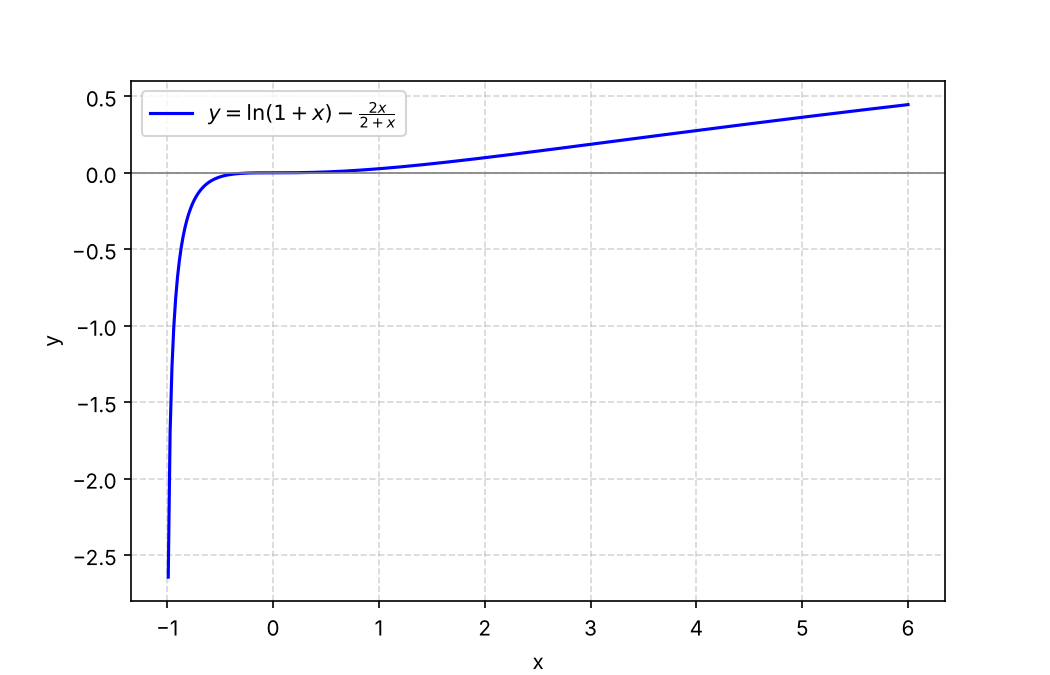
\includegraphics[width=0.60\linewidth]{figs/Q13.png}
    \caption{$y = \ln\brak{1+x} - \frac{2x}{2+x}$ is increasing}
    \label{fig:EE26BTECH11205-13}
\end{figure}

\item
Evaluate $\int x^2\tan^{-1}x\,dx$.

\smallskip
\solution Using \eqref{eq:EE26BTECH11205-ibp} with $u = \tan^{-1}x$, $dv = x^2\,dx$,
\begin{align}
	\int x^2\tan^{-1}x\,dx &= \frac{x^3}{3}\tan^{-1}x - \frac{1}{3}\int\frac{x^3}{1+x^2}\,dx
	\\
	\frac{x^3}{1+x^2} &= x - \frac{x}{1+x^2} \implies \int\frac{x^3}{1+x^2}\,dx = \frac{x^2}{2} - \frac{1}{2}\ln\brak{1+x^2}
\end{align}
Therefore
\begin{align}
	\int x^2\tan^{-1}x\,dx = \frac{x^3}{3}\tan^{-1}x - \frac{x^2}{6} + \frac{1}{6}\ln\brak{1+x^2} + c
\end{align}
\par\medskip\centerline{OR}\smallskip
Evaluate $\int\frac{3x-1}{\brak{x+2}^2}\,dx$.

\smallskip
\solution Since $3x - 1 = 3\brak{x+2} - 7$,
\begin{align}
	\int\frac{3x-1}{\brak{x+2}^2}\,dx = \int\brak{\frac{3}{x+2} - \frac{7}{\brak{x+2}^2}}dx = 3\ln\abs{x+2} + \frac{7}{x+2} + c
\end{align}
The following code verifies both results by differentiation
\begin{lstlisting}[frame=single, basicstyle=\rmfamily, escapeinside={(*@}{@*)}]
(*@\makebox[\dimexpr\linewidth-2\fboxsep-2\fboxrule\relax][c]{codes/Q14.py}@*)
\end{lstlisting}

\item
Solve the differential equation $\sbrak{\frac{e^{-2\sqrt{x}}}{\sqrt{x}} - \frac{y}{\sqrt{x}}}\frac{dx}{dy} = 1$, $x \neq 0$.

\smallskip
\solution The equation requires $x>0$ and $\frac{dx}{dy} \neq 0$, so it can be written as
\begin{align}
	\frac{dy}{dx} + \frac{1}{\sqrt{x}}y = \frac{e^{-2\sqrt{x}}}{\sqrt{x}}
\end{align}
The integrating factor is $\mu = e^{\int x^{-1/2}dx} = e^{2\sqrt{x}}$. From \eqref{eq:EE26BTECH11205-linode},
\begin{align}
	\frac{d}{dx}\brak{ye^{2\sqrt{x}}} = \frac{1}{\sqrt{x}} \implies ye^{2\sqrt{x}} = 2\sqrt{x} + C
\end{align}
Hence
\begin{align}
	y = \brak{2\sqrt{x} + C}e^{-2\sqrt{x}}
\end{align}
The following code verifies the solution
\begin{lstlisting}[frame=single, basicstyle=\rmfamily, escapeinside={(*@}{@*)}]
(*@\makebox[\dimexpr\linewidth-2\fboxsep-2\fboxrule\relax][c]{codes/Q15.py}@*)
\end{lstlisting}

\item
Solve the differential equation $3e^x\tan y\,dx + \brak{2-e^x}\sec^2y\,dy = 0$, given that $y = \frac{\pi}{4}$ when $x = 0$.

\smallskip
\solution Separating the variables,
\begin{align}
	\frac{3e^x}{2-e^x}dx + \frac{\sec^2y}{\tan y}dy = 0
\end{align}
From \eqref{eq:EE26BTECH11205-sepode},
\begin{align}
	-3\ln\abs{2-e^x} + \ln\abs{\tan y} = \ln\abs{C} \implies \tan y = C\brak{2-e^x}^3
\end{align}
At $x = 0$, $y = \frac{\pi}{4}$: $1 = C\brak{1}^3$, so $C = 1$. Hence
\begin{align}
	\tan y = \brak{2-e^x}^3 \implies y = \tan^{-1}\brak{\brak{2-e^x}^3}
\end{align}
which is valid for $e^x < 2$, the interval containing $x = 0$.

\smallskip
The following code compares a numerical solution of the differential equation with this result
\begin{lstlisting}[frame=single, basicstyle=\rmfamily, escapeinside={(*@}{@*)}]
(*@\makebox[\dimexpr\linewidth-2\fboxsep-2\fboxrule\relax][c]{codes/Q16.py}@*)
\end{lstlisting}

\item
If $\vec{\alpha} = 3\hat{\imath} + 4\hat{\jmath} + 5\hat{k}$ and $\vec{\beta} = 2\hat{\imath} + \hat{\jmath} - 4\hat{k}$, then express $\vec{\beta}$ in the form $\vec{\beta} = \vec{\beta}_1 + \vec{\beta}_2$, where $\vec{\beta}_1$ is parallel to $\vec{\alpha}$ and $\vec{\beta}_2$ is perpendicular to $\vec{\alpha}$.

\smallskip
\solution Here
\begin{align}
	\vec{\alpha} = \myvec{3 \\ 4 \\ 5},\quad \vec{\beta} = \myvec{2 \\ 1 \\ -4}
	\\
	\vec{\alpha}^{\top}\vec{\alpha} = 50,\quad \vec{\alpha}^{\top}\vec{\beta} = 6 + 4 - 20 = -10
\end{align}
From \eqref{eq:EE26BTECH11205-proj},
\begin{align}
	\vec{\beta}_1 = \frac{\vec{\alpha}^{\top}\vec{\beta}}{\vec{\alpha}^{\top}\vec{\alpha}}\vec{\alpha} = -\frac{1}{5}\myvec{3 \\ 4 \\ 5} = \myvecf{-\frac{3}{5} \\ -\frac{4}{5} \\ -1}
	\\
	\vec{\beta}_2 = \vec{\beta} - \vec{\beta}_1 = \myvecf{\frac{13}{5} \\ \frac{9}{5} \\ -3}
\end{align}
Check: $\vec{\alpha}^{\top}\vec{\beta}_2 = \frac{39 + 36 - 75}{5} = 0$. Hence
\begin{align}
	\vec{\beta} = \brak{-\frac{3}{5}\hat{\imath} - \frac{4}{5}\hat{\jmath} - \hat{k}} + \brak{\frac{13}{5}\hat{\imath} + \frac{9}{5}\hat{\jmath} - 3\hat{k}}
\end{align}
The following code verifies the solution
\begin{lstlisting}[frame=single, basicstyle=\rmfamily, escapeinside={(*@}{@*)}]
(*@\makebox[\dimexpr\linewidth-2\fboxsep-2\fboxrule\relax][c]{codes/Q17.py}@*)
\end{lstlisting}

\item
Find the vector and Cartesian equations of the line passing through the point $\vec{P} = \brak{1,2,3}$ and parallel to the planes $\vec{r}\cdot\brak{\hat{\imath} - \hat{\jmath} + 2\hat{k}} = 5$ and $\vec{r}\cdot\brak{3\hat{\imath} + \hat{\jmath} + \hat{k}} = 6$.

\smallskip
\solution The normal vectors are
\begin{align}
	\vec{n}_1 = \myvec{1 \\ -1 \\ 2}, \quad \vec{n}_2 = \myvec{3 \\ 1 \\ 1}
\end{align}
From \eqref{eq:EE26BTECH11205-line-planes}, $\vec{d}$ lies in the null space of
\begin{align}
	\myvec{1 & -1 & 2 \\ 3 & 1 & 1} \xrightarrow{\vec{R}_2 \to \vec{R}_2 - 3\vec{R}_1} \myvec{1 & -1 & 2 \\ 0 & 4 & -5}
\end{align}
Taking $d_3 = 4$ gives $d_2 = 5$, $d_1 = d_2 - 2d_3 = -3$, which agrees with
\begin{align}
	\vec{d} = \vec{n}_1\times\vec{n}_2 = \myvec{-3 \\ 5 \\ 4}
\end{align}
The vector equation of the line is
\begin{align}
	\vec{r} = \brak{\hat{\imath} + 2\hat{\jmath} + 3\hat{k}} + \lambda\brak{-3\hat{\imath} + 5\hat{\jmath} + 4\hat{k}}
\end{align}
and the Cartesian equation is
\begin{align}
	\frac{x-1}{-3} = \frac{y-2}{5} = \frac{z-3}{4}
\end{align}

\item
A pair of dice is thrown 4 times. If getting a doublet is considered a success, find the probability distribution of the number of successes and hence find its mean.

\smallskip
\solution A doublet occurs in $6$ of the $36$ outcomes, so $p = \frac{1}{6}$ and $q = \frac{5}{6}$. The number of successes $X$ in $n = 4$ independent throws follows \eqref{eq:EE26BTECH11205-binom-pmf},
\begin{align}
	\pr{X=k} = \comb{4}{k}\brak{\frac{1}{6}}^k\brak{\frac{5}{6}}^{4-k}
\end{align}
\begin{center}
\renewcommand{\arraystretch}{2.2}
\begin{tabular}{c|c|c|c|c|c}
$k$ & $0$ & $1$ & $2$ & $3$ & $4$ \\ \hline
$\pr{X=k}$ & $\frac{625}{1296}$ & $\frac{500}{1296}$ & $\frac{150}{1296}$ & $\frac{20}{1296}$ & $\frac{1}{1296}$
\end{tabular}
\end{center}
The probabilities add up to $\frac{1296}{1296} = 1$. From \eqref{eq:EE26BTECH11205-binom-mean},
\begin{align}
	\mean{X} = np = 4\brak{\frac{1}{6}} = \frac{2}{3}
\end{align}
The following code verifies the solution (including a simulation) and generates \figref{fig:EE26BTECH11205-19}.
\begin{lstlisting}[frame=single, basicstyle=\rmfamily, escapeinside={(*@}{@*)}]
(*@\makebox[\dimexpr\linewidth-2\fboxsep-2\fboxrule\relax][c]{codes/Q19.py}@*)
\end{lstlisting}
\begin{figure}[H]
    \centering
    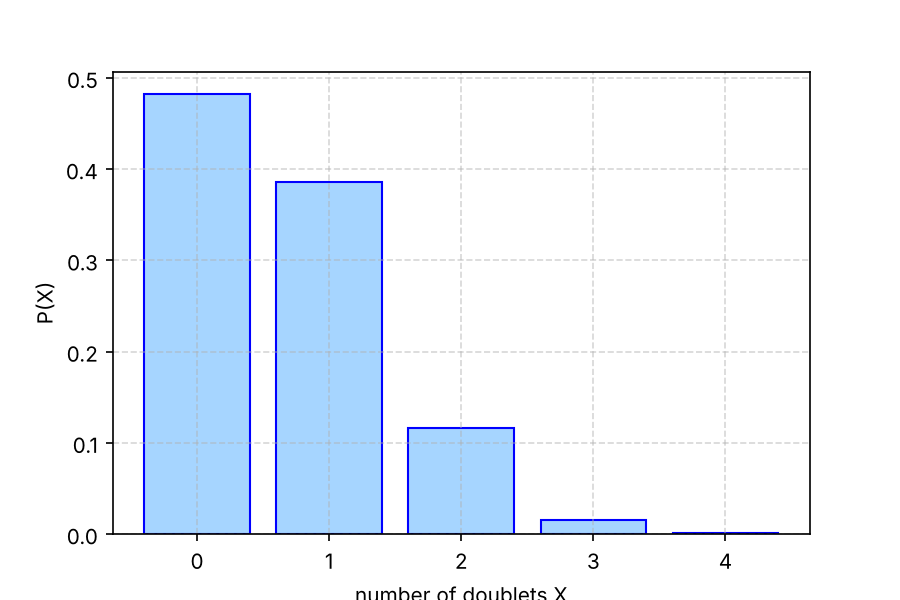
\includegraphics[width=0.55\linewidth]{figs/Q19.png}
    \caption{Probability distribution of the number of doublets}
    \label{fig:EE26BTECH11205-19}
\end{figure}

%--------------------------------------------------------------------- Section C
\item
Using matrices, solve the following system of equations: $x - y + z = 4$, $2x + y - 3z = 0$, $x + y + z = 2$.

\smallskip
\solution From \eqref{eq:EE26BTECH11205-linsys},
\begin{align}
	\myvec{1 & -1 & 1 \\ 2 & 1 & -3 \\ 1 & 1 & 1}\myvec{x \\ y \\ z} = \myvec{4 \\ 0 \\ 2}
	\\
	\mydet{\vec{A}} = 1\brak{1+3} + 1\brak{2+3} + 1\brak{2-1} = 10 \neq 0
\end{align}
so the solution is unique. Gaussian elimination on the augmented matrix gives
\begin{align}
	\myvec{1 & -1 & 1 & 4 \\ 2 & 1 & -3 & 0 \\ 1 & 1 & 1 & 2}
	\xrightarrow[\vec{R}_3 \to \vec{R}_3 - \vec{R}_1]{\vec{R}_2 \to \vec{R}_2 - 2\vec{R}_1}
	\myvec{1 & -1 & 1 & 4 \\ 0 & 3 & -5 & -8 \\ 0 & 2 & 0 & -2}
\end{align}
The last row gives $y = -1$. Then $3\brak{-1} - 5z = -8 \implies z = 1$ and $x + 1 + 1 = 4 \implies x = 2$. Hence
\begin{align}
	\myvec{x \\ y \\ z} = \myvec{2 \\ -1 \\ 1}
\end{align}
\par\medskip\centerline{OR}\smallskip
If $\vec{A}^{-1} = \myvec{3 & -1 & 1 \\ -15 & 6 & -5 \\ 5 & -2 & 2}$ and $\vec{B} = \myvec{1 & 2 & -2 \\ -1 & 3 & 0 \\ 0 & -2 & 1}$, find $\brak{\vec{A}\vec{B}}^{-1}$.

\smallskip
\solution From \eqref{eq:EE26BTECH11205-inv-prod}, $\brak{\vec{A}\vec{B}}^{-1} = \vec{B}^{-1}\vec{A}^{-1}$. Here $\mydet{\vec{B}} = 1\brak{3} - 2\brak{-1} - 2\brak{2} = 1$ and, from \eqref{eq:EE26BTECH11205-adjugate}, the matrix of cofactors is
\begin{align}
	\vec{C} = \myvec{3 & 1 & 2 \\ 2 & 1 & 2 \\ 6 & 2 & 5} \implies \vec{B}^{-1} = \vec{C}^{\top} = \myvec{3 & 2 & 6 \\ 1 & 1 & 2 \\ 2 & 2 & 5}
\end{align}
Therefore
\begin{align}
	\brak{\vec{A}\vec{B}}^{-1} = \myvec{3 & 2 & 6 \\ 1 & 1 & 2 \\ 2 & 2 & 5}\myvec{3 & -1 & 1 \\ -15 & 6 & -5 \\ 5 & -2 & 2} = \myvec{9 & -3 & 5 \\ -2 & 1 & 0 \\ 1 & 0 & 2}
\end{align}
The following code verifies both parts
\begin{lstlisting}[frame=single, basicstyle=\rmfamily, escapeinside={(*@}{@*)}]
(*@\makebox[\dimexpr\linewidth-2\fboxsep-2\fboxrule\relax][c]{codes/Q20.py}@*)
\end{lstlisting}

\item
Show that the altitude of the right circular cone of maximum volume that can be inscribed in a sphere of radius $R$ is $\frac{4R}{3}$.

\smallskip
\solution From \eqref{eq:EE26BTECH11205-cone-vol},
\begin{align}
	V\brak{h} = \frac{\pi}{3}\brak{2Rh^2 - h^3},\quad 0<h<2R
	\\
	V^{\prime}\brak{h} = \frac{\pi}{3}\brak{4Rh - 3h^2} = \frac{\pi}{3}h\brak{4R-3h}
\end{align}
Since $h>0$, $V^{\prime}\brak{h} = 0$ gives $h = \frac{4R}{3}$ as the only critical point, and
\begin{align}
	V^{\prime\prime}\brak{h} = \frac{\pi}{3}\brak{4R - 6h} \implies V^{\prime\prime}\brak{\frac{4R}{3}} = -\frac{4\pi R}{3} < 0
\end{align}
From \eqref{eq:EE26BTECH11205-second-deriv}, $V$ is maximum at $h = \frac{4R}{3}$. Since $V\to0$ as $h\to0$ or $h\to2R$, this is the global maximum, with $V_{\max} = \frac{32\pi R^3}{81}$.

\smallskip
The following code verifies the solution and generates \figref{fig:EE26BTECH11205-21}.
\begin{lstlisting}[frame=single, basicstyle=\rmfamily, escapeinside={(*@}{@*)}]
(*@\makebox[\dimexpr\linewidth-2\fboxsep-2\fboxrule\relax][c]{codes/Q21.py}@*)
\end{lstlisting}
\begin{figure}[H]
    \centering
    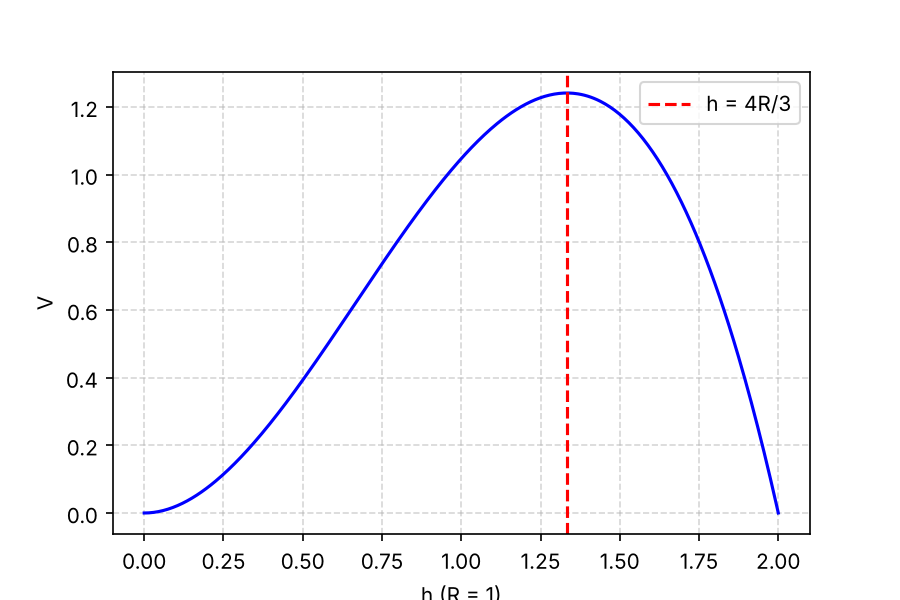
\includegraphics[width=0.55\linewidth]{figs/Q21.png}
    \caption{Volume of the inscribed cone versus its height ($R=1$)}
    \label{fig:EE26BTECH11205-21}
\end{figure}

\item
Find the area of the region in the first quadrant enclosed by the $x$-axis, the line $x = \sqrt{3}\,y$ and the circle $x^2 + y^2 = 4$.

\smallskip
\solution The line and the circle meet where $3y^2 + y^2 = 4$, that is, at $\brak{\sqrt{3},1}$. The region is bounded by the line for $0\le x\le\sqrt{3}$ and by the circle for $\sqrt{3}\le x\le2$. From \eqref{eq:EE26BTECH11205-area-int},
\begin{align}
	A &= \int_{0}^{\sqrt{3}}\frac{x}{\sqrt{3}}\,dx + \int_{\sqrt{3}}^{2}\sqrt{4-x^2}\,dx
	\\
	&= \frac{\sqrt{3}}{2} + \sbrak{\frac{x}{2}\sqrt{4-x^2} + 2\sin^{-1}\frac{x}{2}}_{\sqrt{3}}^{2}
	\\
	&= \frac{\sqrt{3}}{2} + \brak{\pi - \frac{\sqrt{3}}{2} - \frac{2\pi}{3}} = \frac{\pi}{3}
\end{align}
This agrees with the sector of radius $2$ and angle $\frac{\pi}{6}$: $\frac{1}{2}\brak{4}\frac{\pi}{6} = \frac{\pi}{3}$.

\smallskip
The following code verifies the solution and generates \figref{fig:EE26BTECH11205-22}.
\begin{lstlisting}[frame=single, basicstyle=\rmfamily, escapeinside={(*@}{@*)}]
(*@\makebox[\dimexpr\linewidth-2\fboxsep-2\fboxrule\relax][c]{codes/Q22.py}@*)
\end{lstlisting}
\begin{figure}[H]
    \centering
    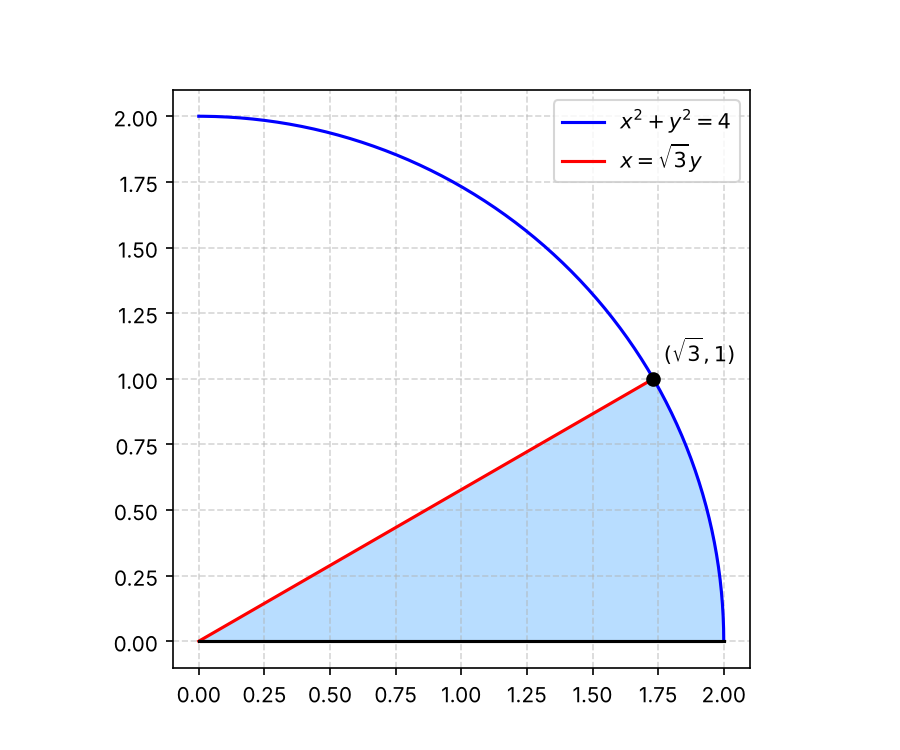
\includegraphics[width=0.55\linewidth]{figs/Q22.png}
    \caption{Region bounded by the $x$-axis, $x=\sqrt{3}y$ and $x^2+y^2=4$}
    \label{fig:EE26BTECH11205-22}
\end{figure}

\item
Evaluate $\int_{1}^{3}\brak{x^2+x}\,dx$ as a limit of a sum.

\smallskip
\solution Here $a = 1$, $b = 3$, $h = \frac{2}{n}$ and $f\brak{1+ih} = \brak{1+ih}^2 + \brak{1+ih} = 2 + 3ih + i^2h^2$. From \eqref{eq:EE26BTECH11205-riemann} and \eqref{eq:EE26BTECH11205-sums},
\begin{align}
	S_n &= h\sbrak{2n + 3h\frac{n\brak{n+1}}{2} + h^2\frac{n\brak{n+1}\brak{2n+1}}{6}}
	\\
	&= 4 + \frac{6\brak{n+1}}{n} + \frac{4\brak{n+1}\brak{2n+1}}{3n^2} = \frac{38}{3} + \frac{10}{n} + \frac{4}{3n^2}
\end{align}
Hence
\begin{align}
	\int_{1}^{3}\brak{x^2+x}\,dx = \lim_{n\to\infty}S_n = \frac{38}{3}
\end{align}
\par\medskip\centerline{OR}\smallskip
Evaluate $\int_{0}^{\pi/4}\frac{\cos^2x}{\cos^2x + 4\sin^2x}\,dx$.

\smallskip
\solution From \eqref{eq:EE26BTECH11205-tan-sub} with $t = \tan x$ and $k = 4$,
\begin{align}
	\int_{0}^{\pi/4}\frac{\cos^2x}{\cos^2x + 4\sin^2x}\,dx = \int_{0}^{1}\frac{dt}{\brak{1+t^2}\brak{1+4t^2}}
\end{align}
Using partial fractions, $\frac{1}{\brak{1+t^2}\brak{1+4t^2}} = \frac{-1/3}{1+t^2} + \frac{4/3}{1+4t^2}$,
\begin{align}
	\int_{0}^{1}\brak{\frac{-1/3}{1+t^2} + \frac{4/3}{1+4t^2}}dt = \sbrak{-\frac{1}{3}\tan^{-1}t + \frac{2}{3}\tan^{-1}\brak{2t}}_{0}^{1}
	\\
	= \frac{2}{3}\tan^{-1}2 - \frac{\pi}{12}
\end{align}
which is approximately $0.4763$. The following code verifies both parts
\begin{lstlisting}[frame=single, basicstyle=\rmfamily, escapeinside={(*@}{@*)}]
(*@\makebox[\dimexpr\linewidth-2\fboxsep-2\fboxrule\relax][c]{codes/Q23.py}@*)
\end{lstlisting}

\item
Find the vector equation of the plane passing through the points $\brak{2,1,-1}$ and $\brak{-1,3,4}$ and perpendicular to the plane $x - 2y + 4z = 10$. Also show that the plane thus obtained contains the line $\vec{r} = -\hat{\imath} + 3\hat{\jmath} + 4\hat{k} + \lambda\brak{3\hat{\imath} - 2\hat{\jmath} - 5\hat{k}}$.

\smallskip
\solution Let
\begin{align}
	\vec{P}_1 = \myvec{2 \\ 1 \\ -1}, \quad \vec{P}_2 = \myvec{-1 \\ 3 \\ 4}, \quad \vec{n}_0 = \myvec{1 \\ -2 \\ 4}
\end{align}
From \eqref{eq:EE26BTECH11205-plane-pts},
\begin{align}
	\vec{n} &= \brak{\vec{P}_2 - \vec{P}_1}\times\vec{n}_0 = \myvec{-3 \\ 2 \\ 5}\times\myvec{1 \\ -2 \\ 4}
	\\
	&= \myvec{8+10 \\ 5+12 \\ 6-2} = \myvec{18 \\ 17 \\ 4}
	\\
	\vec{n}^{\top}\vec{P}_1 &= 36 + 17 - 4 = 49
\end{align}
The vector equation of the plane is
\begin{align}
	\vec{r}\cdot\brak{18\hat{\imath} + 17\hat{\jmath} + 4\hat{k}} = 49
\end{align}
Check: $\vec{n}^{\top}\vec{P}_2 = -18 + 51 + 16 = 49$. For the given line,
\begin{align}
	\vec{A}_0 = \myvec{-1 \\ 3 \\ 4}, \quad \vec{d} = \myvec{3 \\ -2 \\ -5}
	\\
	\vec{n}^{\top}\vec{A}_0 = 49,\quad \vec{n}^{\top}\vec{d} = 54 - 34 - 20 = 0
\end{align}
Hence the line passes through a point of the plane and is parallel to it, so the plane contains the line.

\smallskip
The following code verifies the solution
\begin{lstlisting}[frame=single, basicstyle=\rmfamily, escapeinside={(*@}{@*)}]
(*@\makebox[\dimexpr\linewidth-2\fboxsep-2\fboxrule\relax][c]{codes/Q24.py}@*)
\end{lstlisting}

\item
A company produces soft drinks, and a contract requires that a minimum of $80$ units of chemical A and $60$ units of chemical B go into each bottle. The chemicals are available in prepared mix packets from two suppliers. A packet from supplier S has $4$ units of A and $2$ units of B and costs \rupee~$10$. A packet from supplier T has $1$ unit of A and $1$ unit of B and costs \rupee~$4$. How many packets from S and T should the company purchase to honour the contract and yet minimize the cost? Make an LPP and solve it graphically.

\smallskip
\solution Let $\vec{x} = \myvec{x \\ y}$, where $x$ and $y$ are the numbers of packets from S and T. The LPP is
\begin{align}
	\min_{\vec{x}}\; Z = \myvec{10 & 4}\vec{x} \quad \text{s.t.} \quad \myvec{4 & 1 \\ 2 & 1}\vec{x} \ge \myvec{80 \\ 60},\quad \vec{x} \ge \vec{0}
\end{align}
The lines $4x + y = 80$ and $2x + y = 60$ meet at $\brak{10,40}$. The feasible region in \figref{fig:EE26BTECH11205-25} is unbounded, with corner points
\begin{center}
\renewcommand{\arraystretch}{1.6}
\begin{tabular}{c|c|c|c}
Corner point & $\brak{0,80}$ & $\brak{10,40}$ & $\brak{30,0}$ \\ \hline
$Z = 10x+4y$ & $320$ & $260$ & $300$
\end{tabular}
\end{center}
Since $Z \ge 0$ on the feasible region, from \eqref{eq:EE26BTECH11205-lpp} the minimum is attained at a corner point. This can also be seen directly:
\begin{align}
	10x + 4y = \brak{4x+y} + 3\brak{2x+y} \ge 80 + 3\brak{60} = 260
\end{align}
for every feasible point, with equality at $\brak{10,40}$. Hence the company should buy $10$ packets from S and $40$ packets from T, at the minimum cost of \rupee~$260$.

\smallskip
The following code solves the LPP and generates \figref{fig:EE26BTECH11205-25}.
\begin{lstlisting}[frame=single, basicstyle=\rmfamily, escapeinside={(*@}{@*)}]
(*@\makebox[\dimexpr\linewidth-2\fboxsep-2\fboxrule\relax][c]{codes/Q25.py}@*)
\end{lstlisting}
\begin{figure}[H]
    \centering
    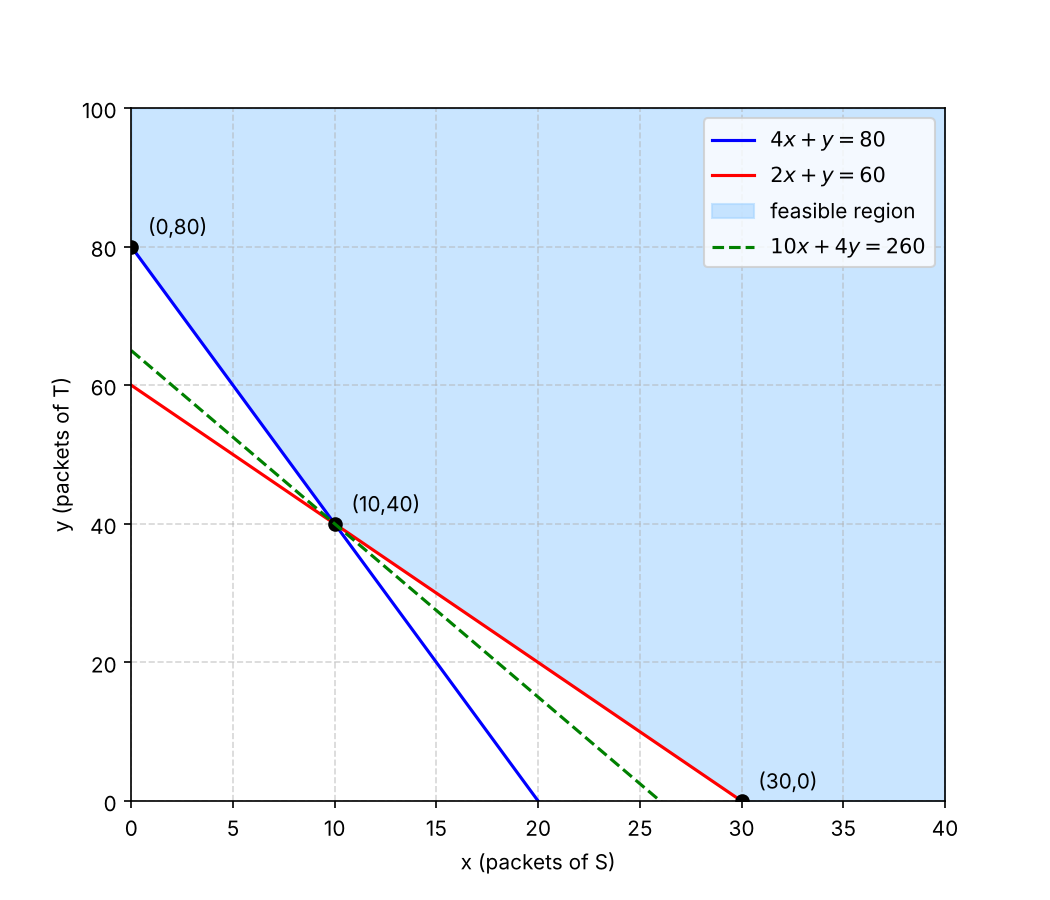
\includegraphics[width=0.60\linewidth]{figs/Q25.png}
    \caption{Feasible region and the optimal corner point $\brak{10,40}$}
    \label{fig:EE26BTECH11205-25}
\end{figure}

\item
In a certain college, $4\%$ of boys and $1\%$ of girls are taller than $1.75$ metres. Furthermore, $60\%$ of the students in the college are girls. A student is selected at random from the college and is found to be taller than $1.75$ metres. Find the probability that the selected student is a girl.

\smallskip
\solution Let $G$: the student is a girl, $B$: the student is a boy, and $T$: the student is taller than $1.75$ m. Then
\begin{align}
	\pr{G} = 0.6,\quad \pr{B} = 0.4,\quad \pr{T|G} = 0.01,\quad \pr{T|B} = 0.04
\end{align}
From \eqref{eq:EE26BTECH11205-bayes},
\begin{align}
	\pr{G|T} = \frac{\pr{G}\pr{T|G}}{\pr{G}\pr{T|G} + \pr{B}\pr{T|B}} = \frac{0.006}{0.006 + 0.016} = \frac{6}{22} = \frac{3}{11}
\end{align}
\end{enumerate}
